\chapter{Le mécanisme de Higgs : comment un boson de jauge acquiert une masse}

Nous réunissons maintenant les deux idées développées au cours de la leçon précédente. Un champ scalaire complexe dont la symétrie globale \(U(1)\) est brisée comporte une oscillation radiale massive et une oscillation angulaire sans masse. Une théorie localement invariante \(U(1)\) comporte un champ de jauge sans masse. Lorsque le champ scalaire est chargé et que sa valeur d’équilibre est non nulle, on ne peut pas simplement juxtaposer ces deux énoncés. Le mode angulaire et le champ de jauge se combinent : le champ de jauge devient massif, le boson de Goldstone apparent cesse d’être une particule indépendante, et le mode radial de Higgs subsiste.

Le photon nous servira de modèle de boson de jauge, mais pas de conclusion physique. La symétrie électromagnétique \(U(1)\) n’est pas brisée dans le vide ; le photon réel est donc sans masse. Le même mécanisme agit sur les bosons \(W^\pm\) et \(Z\) dans la théorie électrofaible, où le groupe de jauge et le multiplet scalaire sont plus complexes. Le modèle abélien met le mécanisme en évidence sans le dissimuler sous la théorie des groupes.

\begin{classroomqa}\audiencequestion{La discussion précédente signifiait-elle que le mécanisme de Higgs donne une masse au photon réel ?\lecturetimestamp{00:00:23}}\lecturerresponse{Non. Nous demandons ce qui se passerait \emph{si} le \(U(1)\) associé au photon se trouvait dans une phase brisée. Ce photon hypothétique deviendrait massif. Le vide électromagnétique réel n’est pas dans cette phase ; en physique des particules, le mécanisme s’applique plutôt aux masses des bosons \(W\) et \(Z\).}\end{classroomqa}

La symétrie associée à la conservation de la charge électrique est la rotation de phase
\begin{equation}
  \phi(x)\longmapsto e^{i\theta}\phi(x),
\end{equation}une rotation interne appelée \(U(1)\). Un supraconducteur fournit un analogue réel de la phase brisée. À l’intérieur, le champ électromagnétique a une profondeur de pénétration finie et se comporte, à plusieurs égards importants, comme un champ massif. À l’extérieur, le photon ordinaire sans masse réapparaît.

\section{Ce que signifie la masse pour un champ}

\subsection{Relation de dispersion et écart à quantité de mouvement nulle}

Il convient de préciser ce que nous entendons par masse avant d’introduire le champ de Higgs. Pour une onde,
\begin{equation}
  E=\hbar\omega,
  \qquad
  p=\hbar k,
  \label{eq:l08-quantum-wave}
\end{equation}
un diagramme \((E,p)\) et un diagramme \((\omega,k)\) contiennent donc la même information, à des facteurs de \(\hbar\) près. Dans le vide, une excitation relativiste sans masse vérifie
\begin{equation}
  E=c|p|,
  \qquad
  \omega=c|k|.
  \label{eq:l08-massless-dispersion}
\end{equation}
Les deux signes de \(k\) distinguent des sens de propagation opposés. L’essentiel est que \(\omega\) tende vers zéro lorsque \(k\) tend vers zéro.

Une particule relativiste massive vérifie
\begin{equation}
  E^2=c^2p^2+m^2c^4.
  \label{eq:l08-massive-dispersion}
\end{equation}
Dans les unités \(c=\hbar=1\),
\begin{equation}
  \omega^2=k^2+m^2.
\end{equation}
Pour \(k=0\), l’énergie vaut \(E=mc^2\), ou simplement \(m\) en unités naturelles. La masse est donc l’écart d’énergie non nul du mode à quantité de mouvement nulle.

\begin{figure}[htbp]\centering
\begin{adjustbox}{max width=\linewidth}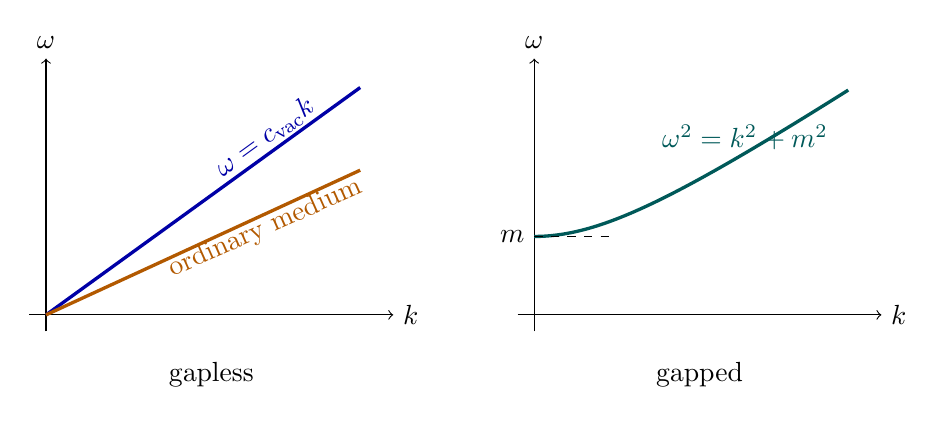
\begin{tikzpicture}[x=1.05cm,y=1.05cm]
  \begin{scope}
    \draw[->] (-0.2,0) -- (4.2,0) node[right] {\(k\)};
    \draw[->] (0,-0.2) -- (0,3.1) node[above] {\(\omega\)};
    \draw[very thick,blue!65!black] (0,0) -- (3.8,2.75);
    \draw[very thick,orange!70!black] (0,0) -- (3.8,1.75);
    \node[blue!65!black,rotate=36] at (2.65,2.15)
      {\(\omega=c_{\rm vac}k\)};
    \node[orange!70!black,rotate=24] at (2.65,1.05)
      {ordinary medium};
    \node[below] at (2,-0.45) {gapless};
  \end{scope}
  \begin{scope}[xshift=6.2cm]
    \draw[->] (-0.2,0) -- (4.2,0) node[right] {\(k\)};
    \draw[->] (0,-0.2) -- (0,3.1) node[above] {\(\omega\)};
    \draw[very thick,domain=0:3.8,samples=120,smooth,teal!70!black]
      plot (\x,{sqrt(0.9+0.45*\x*\x)});
    \draw[dashed] (0,0.95) -- (1.0,0.95);
    \node[left] at (0,0.95) {\(m\)};
    \node[teal!70!black] at (2.55,2.15)
      {\(\omega^2=k^2+m^2\)};
    \node[below] at (2,-0.45) {gapped};
  \end{scope}
\end{tikzpicture}\end{adjustbox}\caption{La modification de la vitesse de propagation change la pente d’une relation de dispersion sans écart. Donner une masse à l’excitation ouvre un écart non nul en \(k=0\).}\label{fig:l08-dispersion}\end{figure}

Un matériau transparent ordinaire peut réduire la vitesse de phase d’une onde sans créer cet écart de masse relativiste. À une interface, la fréquence incidente reste fixe, tandis que le nombre d’onde s’ajuste à la relation de dispersion du milieu. Modifier la pente ne revient pas à relever l’ordonnée à l’origine.
\editorialnote{Un matériau peut présenter plusieurs branches électromagnétiques, et un plasma ou un milieu résonant peut avoir un écart non nul correspondant à la fréquence plasma. La comparaison faite dans cette leçon porte précisément sur une branche réfractive ordinaire et sur la réponse supraconductrice. Plus généralement, l’absence d’écart signifie que \(\omega(k)\to0\) lorsque \(k\to0\) ; la linéarité exacte n’est pas requise dans tous les milieux non relativistes.}

\begin{classroomqa}\audiencequestion{Un photon acquiert-il une masse chaque fois qu’il traverse de la matière, par exemple un prisme ?\lecturetimestamp{00:03:02}}\lecturerresponse{Non. La réfraction peut modifier la relation entre fréquence et nombre d’onde, et donc la vitesse de propagation, alors que la branche passe toujours par \(\omega=0\) pour \(k=0\). En revanche, une phase supraconductrice donne à la réponse électromagnétique une longueur inverse de pénétration finie, analogue d’une masse.}\end{classroomqa}

\begin{classroomqa}\audiencequestion{Pour une lumière de fréquence fixe qui entre dans du verre, est-ce le nombre d’onde qui change ?\lecturetimestamp{00:09:20}}\lecturerresponse{Oui. L’invariance par translation temporelle à une interface stationnaire maintient la fréquence fixe. La courbe de dispersion ayant une pente différente dans le verre, une même \(\omega\) correspond à un \(k\) différent, et donc à une longueur d’onde différente.}\end{classroomqa}

La pente
\begin{equation}
  v_g=\frac{d\omega}{dk}
\end{equation}
est la vitesse de groupe d’un paquet d’ondes. Si cette pente varie avec \(k\), les différentes composantes de Fourier se déplacent à des vitesses différentes et le paquet se disperse. C’est pourquoi la relation \(\omega(k)\) est appelée relation de \emph{dispersion}.

\begin{classroomqa}\audiencequestion{Comment s’appelle cette courbe, et que représente sa pente ?\lecturetimestamp{00:11:02}}\lecturerresponse{Cette courbe est la relation de dispersion. Sa dérivée \(d\omega/dk\) est la vitesse de groupe. Une pente constante donne la même vitesse à toutes les longueurs d’onde ; une pente variable fait s’étaler un paquet d’ondes. Pour ce qui nous occupe, la distinction décisive est de savoir si la courbe atteint l’origine ou présente un écart.}\end{classroomqa}

\subsection{Une oscillation homogène est une particule au repos}

Le mode \(k=0\) a une longueur d’onde infinie : le champ est décalé de la même quantité partout. Libérons un déplacement homogène. Si le champ oscille à une fréquence non nulle, le quantum correspondant a une énergie au repos non nulle et est massif. S’il n’y a pas de force de rappel dans cette direction, la fréquence s’annule et le mode est sans masse.

Cet énoncé est classique. Il n’exige pas que des particules spatialement séparées soient dans une superposition quantique. Une configuration classique de champ homogène est simplement une même valeur du champ répétée dans tout l’espace.

\begin{classroomqa}\audiencequestion{Si tout un champ est décalé en bloc, est-ce la même chose que l’intrication quantique ?\lecturetimestamp{00:10:04}}\lecturerresponse{Non. Un champ classique homogène constitue une configuration classique unique. L’intrication corrèle différentes possibilités quantiques, comme les configurations de spin haut--bas et bas--haut. Préparer la même valeur du champ en de nombreux points ne crée pas, à lui seul, d’intrication et n’implique pas non plus de réponse causale instantanée.}\end{classroomqa}

Pour un champ réel normalisé canoniquement,
\begin{equation}
  \mathcal L
  =\frac12\partial_\mu\varphi\,\partial^\mu\varphi-V(\varphi),
\end{equation}
développons autour d’un point d’équilibre \(\varphi_0\) :
\begin{equation}
  V(\varphi_0+\eta)
  =V(\varphi_0)
   +\frac12V''(\varphi_0)\eta^2+\cdots.
\end{equation}
Le terme linéaire s’annule au minimum, et l’équation du champ donne
\begin{equation}
  \omega^2=\bm{k}^2+m^2,
  \qquad
  m^2=V''(\varphi_0).
  \label{eq:l08-curvature-mass}
\end{equation}
La masse est donc la courbure du potentiel dans la direction du mouvement. Une direction plate a une courbure nulle et donne un mode sans masse.

\section{Le scalaire complexe brisé}

\subsection{Mouvement radial et angulaire}

Écrivons un scalaire complexe en coordonnées cartésiennes et polaires :
\begin{equation}
  \phi=\phi_R+i\phi_I=\rho e^{i\alpha},
  \qquad
  \phi^*=\phi_R-i\phi_I=\rho e^{-i\alpha}.
  \label{eq:l08-polar-field}
\end{equation}
Le plan complexe est un espace des champs \emph{interne}. En chaque point de l’espace-temps physique \(x\), le couple
\((\phi_R(x),\phi_I(x))\)désigne un point de ce plan interne.
Aucun des deux axes internes n’est une direction du laboratoire.

\begin{figure}[htbp]\centering
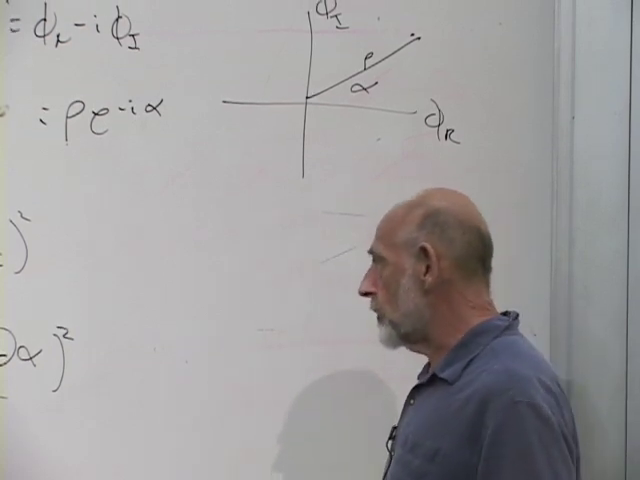
\includegraphics[width=0.72\textwidth]{lecture_08_figure_02.png}\caption{Le scalaire complexe représenté dans son plan \((\phi_R,\phi_I)\) interne. Le rayon vaut \(\rho\), et \(\alpha\) est la phase interne.}\lectureframe{00:24:41}\label{fig:l08-internal-plane}\end{figure}

Le terme cinétique du scalaire devient
\begin{align}
  \partial_\mu\phi^*\,\partial^\mu\phi
  &=
  \partial_\mu\phi_R\,\partial^\mu\phi_R
  +\partial_\mu\phi_I\,\partial^\mu\phi_I
  \notag\\
  &=
  \partial_\mu\rho\,\partial^\mu\rho
  +\rho^2\partial_\mu\alpha\,\partial^\mu\alpha.
  \label{eq:l08-polar-kinetic}
\end{align}
Un potentiel invariant sous \(U(1)\) dépend de
\(\phi^*\phi=\rho^2\), et non de \(\alpha\). Par exemple,
\begin{equation}
  V(\phi)
  =\lambda\left(\phi^*\phi-\frac{f^2}{2}\right)^2,
  \qquad \lambda>0.
  \label{eq:l08-mexican-hat}
\end{equation}
Ses minima forment un cercle. La loi est invariante par rotation commune de phase, mais le choix d’une phase d’équilibre sélectionne un point du cercle.

\begin{figure}[htbp]\centering
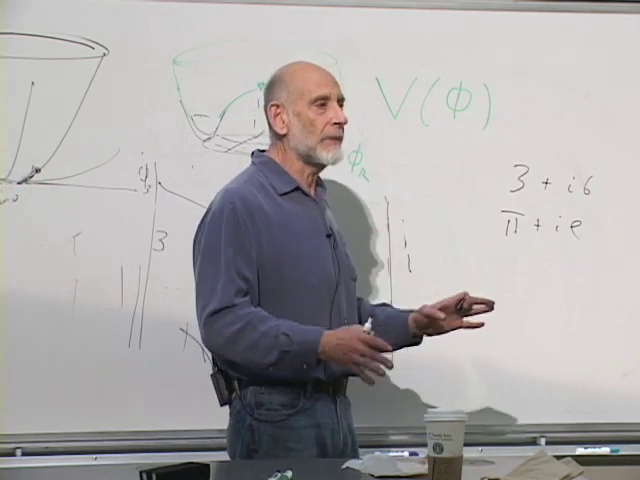
\includegraphics[width=0.78\textwidth]{lecture_08_figure_03.png}\caption{Les croquis au tableau du potentiel radial. Le potentiel est symétrique sous les rotations de la valeur du champ interne, même si le champ lui-même ne se trouve pas nécessairement à l’origine.}\lectureframe{00:34:22}\label{fig:l08-radial-potential-board}\end{figure}

\begin{figure}[htbp]\centering
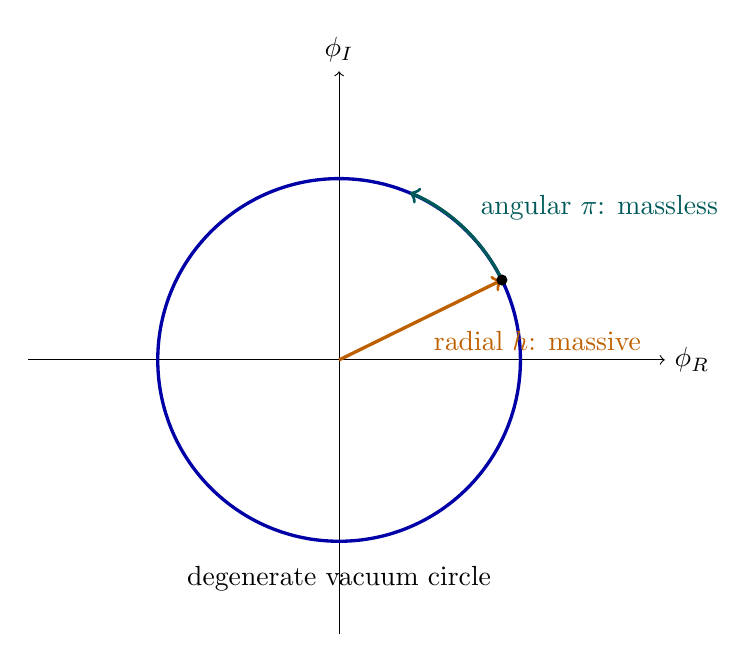
\begin{tikzpicture}[x=0.94cm,y=0.94cm]
  \draw[->] (-4.2,0) -- (4.4,0) node[right] {\(\phi_R\)};
  \draw[->] (0,-3.7) -- (0,3.9) node[above] {\(\phi_I\)};
  \draw[very thick,blue!65!black] (0,0) circle (2.45);
  \draw[->,very thick,orange!75!black] (0,0) -- (2.2,1.08);
  \draw[->,very thick,teal!70!black]
    (2.2,1.08) arc[start angle=26,end angle=67,radius=2.45];
  \node[orange!75!black,below right] at (1.15,0.52)
    {radial \(h\): massive};
  \node[teal!70!black,above right] at (1.78,1.76)
    {angular \(\pi\): massless};
  \fill (2.2,1.08) circle (2pt);
  \node[below] at (0,-2.65) {degenerate vacuum circle};
\end{tikzpicture}\caption{Dans la théorie globale brisée, la courbure est non nulle perpendiculairement au cercle des vides, mais nulle le long de celui-ci. Le mode radial de Higgs est massif ; le mode angulaire de Goldstone est sans masse.}\label{fig:l08-radial-angular}\end{figure}

Posons
\begin{equation}
  \phi(x)=\frac{f+h(x)}{\sqrt2}
           e^{i\pi(x)/f}.
  \label{eq:l08-canonical-polar}
\end{equation}
Au voisinage du vide choisi, \(h\) mesure le déplacement radial et \(\pi\) le déplacement tangentiel, avec des dimensions canoniques. En substituant dans l’équation~\eqref{eq:l08-polar-kinetic}, on obtient
\begin{equation}
  \partial_\mu\phi^*\,\partial^\mu\phi
  =
  \frac12(\partial_\mu h)^2
  +\frac12\left(1+\frac{h}{f}\right)^2
            (\partial_\mu\pi)^2.
  \label{eq:l08-global-expanded}
\end{equation}
Le potentiel de l’équation~\eqref{eq:l08-mexican-hat} fournit
\begin{equation}
  m_h^2=2\lambda f^2,
  \qquad
  m_\pi^2=0.
  \label{eq:l08-global-masses}
\end{equation}
À des énergies très inférieures à \(m_h\), le mouvement radial coûte cher ; nous pouvons donc figer temporairement \(h=0\). Le lagrangien restant ne contient que \(\frac12(\partial\pi)^2\), sans terme en \(\pi^2\). C’est le boson de Goldstone.\editorialnote{À deux reprises, l’explication orale inverse les noms et affirme que l’absorption du boson de Goldstone donne sa masse au boson de Higgs. Le calcul au tableau et la suite de la leçon établissent le résultat voulu : la courbure radiale donne déjà une masse au mode de Higgs, tandis que le boson de jauge acquiert le mode de Goldstone et devient massif.}

\begin{classroomqa}\audiencequestion{Est-ce le seul bris spontané de symétrie dans le modèle standard ?\lecturetimestamp{00:16:39}}\lecturerresponse{La phase de Higgs électrofaible est le mécanisme de brisure de symétrie établi qui nous intéresse ici. La symétrie réelle est \(SU(2)_L\times U(1)_Y\), et non ce seul \(U(1)\) ; la QCD présente aussi d’autres structures du vide, comme la brisure de la symétrie chirale. L’exemple abélien est un modèle volontairement réduit du mécanisme d’acquisition d’une masse par un boson de jauge.}\end{classroomqa}

\begin{classroomqa}\audiencequestion{Le Higgs donne-t-il une masse à toutes les particules, y compris à lui-même ?\lecturetimestamp{00:17:11}}\lecturerresponse{La réponse comporte une distinction : oui et non. La symétrie électrofaible interdit les masses nues des bosons \(W\) et \(Z\) ainsi que des fermions du modèle standard ; leurs masses apparaissent lorsque le champ de Higgs prend une valeur d’équilibre non nulle. La masse radiale du Higgs provient de la courbure de son propre potentiel. D’autres particules hypothétiques peuvent avoir des masses autorisées par la symétrie et sans rapport avec ce mécanisme.}\end{classroomqa}

La leçon associe ces masses autorisées par la symétrie à des particules potentiellement très lourdes et difficiles à observer, et mentionne la matière noire comme exemple possible. C’est une motivation, et non une prédiction de masse.
\editorialnote{L’échelle de masse de la matière noire reste inconnue. L’hypothèse avancée dans la leçon d’une particule d’environ mille masses du proton relève d’une spéculation historique ; ce n’est pas une propriété de la matière noire établie expérimentalement.}

\begin{classroomqa}\audiencequestion{\(\rho\) est-il un rayon physique ou la valeur du champ ? Qu’est-ce qui est exactement symétrique radialement ?\lecturetimestamp{00:33:08}}\lecturerresponse{En chaque point de l’espace-temps, la valeur du champ est un point d’un plan complexe auxiliaire, et \(\rho=|\phi|\) est la distance de ce point à l’origine. Le \emph{potentiel} est radialement symétrique dans ce plan interne : tous les points ayant le même \(\rho\) ont la même énergie potentielle. Ce rayon n’est pas une distance dans l’espace ordinaire.}\end{classroomqa}

\begin{classroomqa}\audiencequestion{Une impulsion radiale assez violente pourrait-elle faire franchir au champ le maximum central du potentiel et l’amener de l’autre côté ?
\lecturetimestamp{00:36:00}}\lecturerresponse{En principe, une configuration locale dotée d’une énergie suffisante peut franchir la barrière. Pour qu’un champ macroscopique homogène la franchisse, il faudrait une énergie énorme ; une perturbation violente générique dissiperait son énergie dans de nombreux modes du champ au lieu d’atteindre de façon cohérente le point opposé. L’approximation de basse énergie fige précisément \(\rho\), car de telles excursions radiales y sont inaccessibles.}\end{classroomqa}

\section{Pourquoi le plan complexe n’est pas l’espace-temps}

La distinction entre coordonnées physiques et coordonnées internes mérite que l’on s’y arrête comme dans la leçon. Un champ est dit scalaire parce qu’il reste invariant sous les rotations des axes de coordonnées physiques. Les deux champs scalaires réels \(\phi_R(x)\) et \(\phi_I(x)\) restent des scalaires sous ces rotations. On peut les regrouper en un nombre complexe, mais cette notation ne les transforme pas en composantes d’un vecteur spatial.

Une transformation globale \(U(1)\) fait tourner les \emph{valeurs} du champ :
\begin{equation}
\begin{aligned}
  \phi(x)&\longmapsto e^{i\theta}\phi(x),
  \\
  \rho(x)&\longmapsto\rho(x),
  \\
  \alpha(x)&\longmapsto\alpha(x)+\theta.
\end{aligned}
  \label{eq:l08-global-shift}
\end{equation}
La même constante \(\theta\) est utilisée en tout point de l’espace-temps. Par conséquent, \(\partial_\mu\alpha\) reste inchangé. Il s’agit d’une symétrie du potentiel comme du terme cinétique ordinaire. Dès que l’on autorise \(\theta\) à dépendre de \(x\), la dérivée détecte cette variation et le raisonnement change.

\section{Rendre locale la rotation de phase}

\subsection{La dérivée ordinaire ne convient plus}

Soit
\begin{equation}
  \phi'(x)=e^{i\theta(x)}\phi(x).
  \label{eq:l08-local-phase}
\end{equation}
Alors
\begin{equation}
  \partial_\mu\phi'
  =e^{i\theta}
    \left(\partial_\mu\phi+i\,\partial_\mu\theta\,\phi\right).
  \label{eq:l08-ordinary-derivative-fails}
\end{equation}
Le terme supplémentaire proportionnel à \(\partial_\mu\theta\) empêche \(\partial_\mu\phi\) de se transformer comme \(\phi\). Par conséquent, \(\partial_\mu\phi^*\partial^\mu\phi\) n’est pas invariant sous des rotations de phase locales arbitraires.

\begin{figure}[htbp]\centering
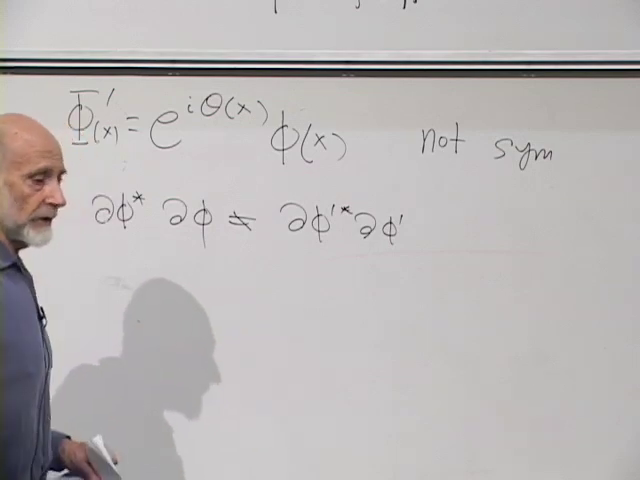
\includegraphics[width=0.78\textwidth]{lecture_08_figure_04.png}\caption{Le tableau présente la transformation locale de phase et montre que le terme faisant intervenir la dérivée ordinaire cesse d’être invariant.}\lectureframe{00:46:49}\label{fig:l08-local-not-symmetry}\end{figure}

Introduisons un potentiel vecteur et adoptons une convention que nous garderons partout :
\begin{equation}
  D_\mu=\partial_\mu+i g A_\mu,
  \qquad
  A_\mu'=A_\mu-\frac1g\partial_\mu\theta.
  \label{eq:l08-covariant-convention}
\end{equation}
On a alors
\begin{align}
  D_\mu'\phi'
  &=
  \left(\partial_\mu+i g A_\mu'\right)
  e^{i\theta}\phi
  \notag\\
  &=
  e^{i\theta}
  \left[
    \partial_\mu\phi+i(\partial_\mu\theta)\phi
    +i g A_\mu\phi-i(\partial_\mu\theta)\phi
  \right]
  \notag\\
  &=e^{i\theta}D_\mu\phi.
  \label{eq:l08-covariant-transform}
\end{align}
Les termes indésirables s’annulent. La dérivée conjuguée est
\begin{equation}
  (D_\mu\phi)^*
  =(\partial_\mu-i g A_\mu)\phi^*,
\end{equation}
et sa phase opposée s’annule dans le produit
\begin{equation}
  (D_\mu\phi)^*D^\mu\phi.
\end{equation}

\begin{classroomqa}\audiencequestion{Dans la leçon précédente, la transformation du champ de jauge était-elle écrite avec le signe opposé ?\lecturetimestamp{00:48:04}}\lecturerresponse{Inverser simultanément le signe dans \(D_\mu\) et celui de la loi de transformation est un simple choix de convention. Avec \(D_\mu=\partial_\mu+i gA_\mu\) et \(\phi'=e^{i\theta}\phi\), la cohérence impose \(A_\mu'=A_\mu-g^{-1}\partial_\mu\theta\). L’autre convention convient tout autant si l’on change tous les signes ensemble.}\end{classroomqa}

\begin{classroomqa}\audiencequestion{L’emploi au tableau d’une forme majuscule ou minuscule de \(\phi\) désigne-t-il un champ différent ?\lecturetimestamp{00:55:02}}\lecturerresponse{Aucune distinction n’est voulue. La variation de la forme de la lettre relève de l’écriture manuscrite ; elle ne représente ni une opération supplémentaire ni un second scalaire. Les distinctions significatives sont la prime, l’étoile de conjugaison complexe et l’indice d’espace-temps.}\end{classroomqa}

\begin{classroomqa}\audiencequestion{La conjugaison complexe est-elle la même opération que la montée ou la descente de l’indice de Lorentz dans le terme cinétique ?
\lecturetimestamp{00:56:50}}\lecturerresponse{Non. L’étoile conjugue le champ complexe interne. Les indices de Lorentz sont montés au moyen de la métrique de l’espace-temps : \(D^\mu=g^{\mu\nu}D_\nu\). Un scalaire de Lorentz nécessite la contraction \((D_\mu\phi)^*D^\mu\phi\) ; ces deux opérations interviennent et remplissent des rôles différents.}\end{classroomqa}

\subsection{Le champ de jauge a sa propre dynamique}

Le tenseur de champ
\begin{equation}
  F_{\mu\nu}=\partial_\mu A_\nu-\partial_\nu A_\mu
  \label{eq:l08-field-strength}
\end{equation}
est invariant de jauge, car les deux dérivées secondes mixtes de \(\theta\) s’annulent. Ses composantes temps--espace contiennent le champ électrique, et ses composantes espace--espace contiennent le champ magnétique. L’électrodynamique scalaire s’écrit donc
\begin{equation}
  \mathcal L
  =(D_\mu\phi)^*D^\mu\phi
  -V(\phi^*\phi)
  -\frac14F_{\mu\nu}F^{\mu\nu}.
  \label{eq:l08-abelian-higgs}
\end{equation}
Le champ chargé considéré ici est bosonique. Ce n’est pas le champ de l’électron, qui est un fermion. Un noyau d’hélium chargé ou un condensat de paires de Cooper illustre la façon dont peut apparaître un degré de liberté bosonique chargé.

Avant la brisure de symétrie, le terme de jauge contient des dérivées de \(A_\mu\), mais aucun terme de masse direct. On pourrait tenter d’ajouter
\begin{equation}
  \frac12m_A^2A_\mu A^\mu,
\end{equation}
mais sous la transformation de l’équation~\eqref{eq:l08-covariant-convention},
\begin{equation}
  A_\mu A^\mu
  \longmapsto
  \left(A_\mu-\frac1g\partial_\mu\theta\right)
  \left(A^\mu-\frac1g\partial^\mu\theta\right),
  \label{eq:l08-bare-mass-fails}
\end{equation}
ce qui n’est pas égal à \(A_\mu A^\mu\). La symétrie locale interdit une masse nue pour le boson de jauge.

\begin{figure}[htbp]\centering
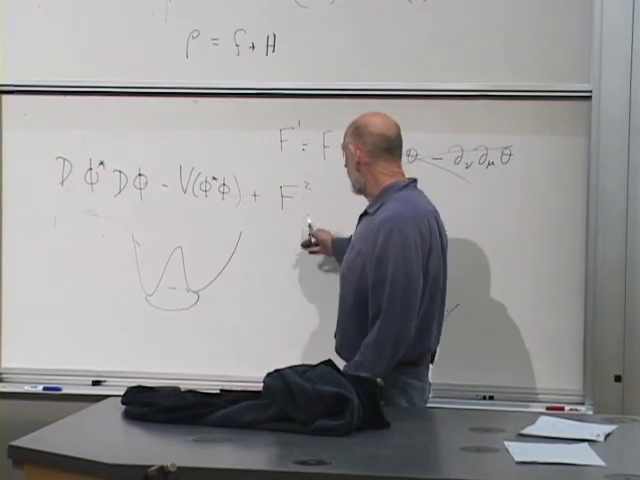
\includegraphics[width=0.76\textwidth]{lecture_08_figure_05.png}\caption{Une étape du calcul vérifiée au tableau met en évidence l’obstacle : sous une transformation de jauge, \(A_\mu A^\mu\) devient un carré contenant \(\partial_\mu\theta\) ; une masse nue du champ vectoriel n’est donc pas invariante.}\lectureframe{01:07:30}\label{fig:l08-bare-mass-board}\end{figure}

\section{Le mécanisme de Higgs}

\subsection{La dérivée covariante produit la masse}

Revenons au potentiel brisé et utilisons la paramétrisation à normalisation canonique
\begin{equation}
  \phi(x)=\frac{f+h(x)}{\sqrt2}
  e^{i\pi(x)/f}.
\end{equation}
Sa dérivée covariante est
\begin{equation}
  D_\mu\phi
  =
  \frac{e^{i\pi/f}}{\sqrt2}
  \left[
    \partial_\mu h
    +i(f+h)
      \left(\frac{\partial_\mu\pi}{f}+gA_\mu\right)
  \right].
  \label{eq:l08-covariant-polar}
\end{equation}
Par conséquent,
\begin{equation}
\begin{aligned}
  (D_\mu\phi)^*D^\mu\phi
  ={}&
  \frac12(\partial_\mu h)^2
  \\
  &+\frac12(f+h)^2
    \left(\frac{\partial_\mu\pi}{f}+gA_\mu\right)
  \\
  &\hspace{4.2em}\times
    \left(\frac{\partial^\mu\pi}{f}+gA^\mu\right).
\end{aligned}
  \label{eq:l08-higgs-kinetic}
\end{equation}

Le terme décisif apparaît avant tout choix de jauge :
\begin{equation}
  \frac12g^2f^2 A_\mu A^\mu.
  \label{eq:l08-vector-mass-term}
\end{equation}
En le comparant à la forme de Proca \(\frac12m_A^2A_\mu A^\mu\), on trouve
\begin{equation}
  \boxed{m_A=g f}.
  \label{eq:l08-vector-mass}
\end{equation}
Le même développement produit également les interactions \(g^2fh A_\mu A^\mu\) et \(\frac12g^2h^2A_\mu A^\mu\). La masse du vecteur n’est donc pas une violation arbitraire de la symétrie de jauge. Elle provient d’un terme cinétique scalaire invariant de jauge, évalué dans une phase où la valeur d’équilibre \(f\) est non nulle.

\begin{figure}[htbp]\centering
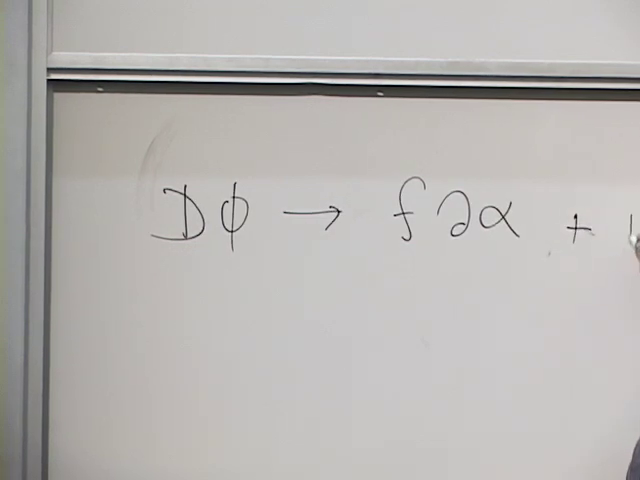
\includegraphics[width=0.78\textwidth]{lecture_08_figure_06.png}\caption{Le tableau isole la contribution \(f^2A^2\) dans \((D\phi)^*(D\phi)\). Les facteurs numériques dépendent de la normalisation du champ scalaire et du couplage de jauge ; avec les équations~\eqref{eq:l08-canonical-polar} et \eqref{eq:l08-covariant-convention}, on obtient \(m_A=gf\).}\lectureframe{01:10:10}\label{fig:l08-generated-mass-board}\end{figure}

Dans la notation employée au tableau, la leçon absorbe \(g\) et plusieurs facteurs de \(\sqrt2\) ; elle alterne donc brièvement entre \(f\), \(2f\) et \(\sqrt2f\) pour identifier la masse. Ces facteurs n’ont pas de signification invariante tant que les normalisations cinétique et potentielle ne sont pas précisées. Le résultat robuste est \(m_A\propto gf\) ; l’équation~\eqref{eq:l08-vector-mass} donne le facteur correspondant à la convention utilisée ici.

\subsection{La phase est absorbée}

Sous une transformation de jauge, la variable de phase se transforme selon
\begin{equation}
  \pi'(x)=\pi(x)+f\,\theta(x).
\end{equation}
Choisissons
\begin{equation}
  \theta(x)=-\frac{\pi(x)}{f}.
  \label{eq:l08-unitary-gauge-choice}
\end{equation}
On a alors \(\pi'=0\). C’est la jauge unitaire, dans laquelle
\begin{equation}
  \phi'(x)=\frac{f+h(x)}{\sqrt2}
\end{equation}
est réel, et l’équation~\eqref{eq:l08-higgs-kinetic} se réduit à
\begin{equation}
  (D_\mu\phi')^*D^\mu\phi'
  =
  \frac12(\partial_\mu h)^2
  +\frac12g^2(f+h)^2A_\mu'A^{\prime\mu}.
  \label{eq:l08-unitary-gauge-lagrangian}
\end{equation}
Le champ de Goldstone angulaire a disparu de la liste des variables indépendantes, tandis que la masse du vecteur subsiste.

La leçon commence par le montrer dans la limite de basse énergie \(\rho=f\), où
\begin{align}
  \phi&=f e^{i\alpha},
  \notag\\
  D_\mu\phi
  &=if e^{i\alpha}
    \left(\partial_\mu\alpha+gA_\mu\right),
  \notag\\
  (D_\mu\phi)^*
  &=-if e^{-i\alpha}
    \left(\partial_\mu\alpha+gA_\mu\right).
  \label{eq:l08-frozen-radius}
\end{align}
Leur produit est
\begin{equation}
  f^2
  \left(\partial_\mu\alpha+gA_\mu\right)
  \left(\partial^\mu\alpha+gA^\mu\right).
\end{equation}
Le choix \(\theta=-\alpha\) laisse \(g^2f^2A_\mu'A^{\prime\mu}\).

\begin{figure}[htbp]\centering
\includegraphics[width=0.82\textwidth]{lecture_08_figure_07.png}\caption{Le calcul complet au tableau à rayon figé : les dérivées covariantes contiennent ensemble la dérivée de phase et le potentiel vecteur. La leçon choisit ensuite \(\theta=-\alpha\), ce qui élimine la phase et laisse le terme de masse du vecteur.}\lectureframe{01:16:20}\label{fig:l08-frozen-radius-board}\end{figure}

\begin{classroomqa}\audiencequestion{Peut-on réécrire tout le lagrangien en variables qui rendent explicite la disparition du mode angulaire ?
\lecturetimestamp{01:13:49}}\lecturerresponse{Oui. En variables polaires, la phase n’apparaît que dans la combinaison invariante de jauge \(\partial_\mu\alpha+gA_\mu\). Une transformation de jauge avec \(\theta=-\alpha\) annule la phase partout où cette jauge est bien définie. Le terme cinétique scalaire devient alors un terme de masse du vecteur, tandis que le terme de force de champ invariant de jauge reste inchangé.}\end{classroomqa}

\begin{classroomqa}\audiencequestion{Les oscillations de \(\alpha\) sont-elles indiscernables des oscillations de jauge ?\lecturetimestamp{01:18:02}}\lecturerresponse{Dans la théorie de jauge, une variation pure de \(\alpha\) compensée par la variation correspondante de \(A_\mu\) est une redescription de jauge, et non une onde physique distincte. La quantité invariante est \(\partial_\mu\alpha+gA_\mu\). Le mode physique représenté par le champ de Goldstone global réapparaît comme polarisation longitudinale du vecteur massif.}\end{classroomqa}

On dit couramment qu’une symétrie de jauge locale est spontanément brisée. Cette formulation est utile sur le plan opérationnel : après fixation de la jauge, le champ scalaire a une valeur du vide non nulle et le spectre comporte un vecteur massif. Au sens strict, toutefois, les transformations de jauge relient des descriptions redondantes, et non des états physiques distincts.
\editorialnote{Une redondance de jauge locale n’est pas brisée au même sens invariant de jauge qu’une symétrie globale. La formulation précise est que la théorie se trouve dans une phase de Higgs. La théorie des perturbations à jauge fixée décrit cette phase par une valeur moyenne non nulle du champ scalaire et le spectre de vecteurs massifs qui en résulte.}

\section{Où est passé le degré de liberté de Goldstone ?}

Aucun élément physique ne peut disparaître simplement parce que nous avons changé de variables. Comptons les degrés de liberté avant et après l’entrée dans la phase de Higgs.

Avant :
\begin{equation}
  \underbrace{2}_{\text{massless vector}}
  +
  \underbrace{2}_{\text{complex scalar}}
  =4.
\end{equation}
Un vecteur sans masse a deux polarisations transverses. Le scalaire complexe a deux composantes réelles, radiale et angulaire.

Après :
\begin{equation}
  \underbrace{3}_{\text{massive vector}}
  +
  \underbrace{1}_{\text{radial Higgs}}
  =4.
  \label{eq:l08-degree-count}
\end{equation}
On peut placer un vecteur massif au repos. Dans son référentiel de repos, aucune direction spatiale n’est privilégiée ; il doit donc avoir trois états de polarisation. Lorsqu’il est en mouvement, deux sont transverses et une est longitudinale. Le mode de Goldstone est devenu cette polarisation longitudinale.

\begin{figure}[htbp]\centering
\begin{adjustbox}{max width=\linewidth}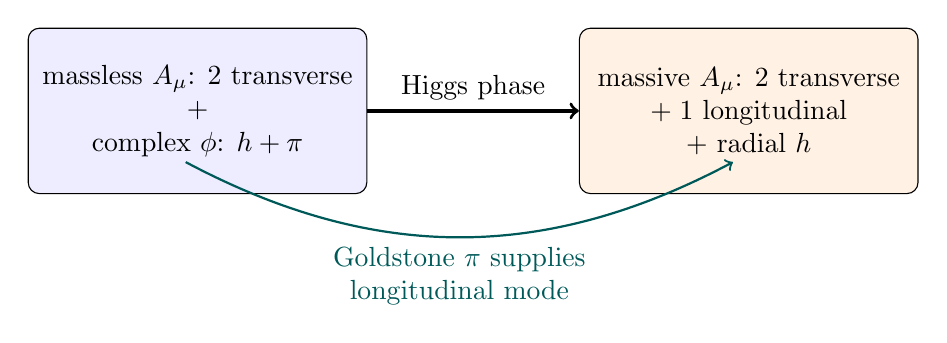
\begin{tikzpicture}[x=1cm,y=1cm]
  \node[draw,rounded corners,fill=blue!7,minimum width=4.3cm,
        minimum height=2.1cm,align=center] (before) at (0,0)
    {massless \(A_\mu\): \(2\) transverse\\
     \(+\)\\
     complex \(\phi\): \(h+\pi\)};
  \node[draw,rounded corners,fill=orange!10,minimum width=4.3cm,
        minimum height=2.1cm,align=center] (after) at (7,0)
    {massive \(A_\mu\): \(2\) transverse\\
     \(+\;1\) longitudinal\\
     \(+\) radial \(h\)};
  \draw[->,very thick] (before) -- node[above]{Higgs phase} (after);
  \draw[->,teal!70!black,thick]
    (-0.15,-0.65) to[bend right=28]
    node[below,align=center]{Goldstone \(\pi\) supplies\\longitudinal mode}
    (6.8,-0.65);
\end{tikzpicture}\end{adjustbox}\caption{Le mécanisme de Higgs réorganise les degrés de liberté physiques au lieu de les détruire.}\label{fig:l08-degree-rearrangement}\end{figure}

\begin{classroomqa}\audiencequestion{Comment le degré de liberté angulaire peut-il disparaître sans que le décompte des degrés de liberté soit violé ?\lecturetimestamp{01:19:13}}\lecturerresponse{Il ne disparaît pas physiquement. Un vecteur sans masse a deux hélicités, car on ne peut pas le placer au repos. Un vecteur massif a trois polarisations, dont une longitudinale. Le mode de Goldstone devient cette troisième polarisation, et le nombre total reste inchangé.}\end{classroomqa}

La leçon propose un test cinématique utile. Imaginons une particule vectorielle massive, ralentissons-la jusqu’à l’arrêt, puis accélérons-la dans une nouvelle direction. Une polarisation transverse par rapport au mouvement initial peut devenir longitudinale par rapport au nouveau mouvement. De même, si une particule massive polarisée circulairement est amenée au repos puis repart en sens opposé, son étiquette d’hélicité s’inverse. Une particule strictement sans masse ne peut pas être soumise à cette expérience, car aucun référentiel inertiel ne peut la placer au repos. Ses deux hélicités forment donc un spectre physique cohérent.

\section{L’analogue supraconducteur}

Dans un supraconducteur conventionnel, les électrons forment des paires de Cooper. Une paire est un boson de charge électrique \(2e\), et le condensat est décrit par un paramètre d’ordre complexe chargé. Lorsque son module est non nul, la combinaison de sa phase et du potentiel vecteur électromagnétique produit le mécanisme d’Anderson--Higgs. Les champs magnétiques statiques décroissent sur la profondeur de pénétration de London au lieu de s’étendre librement dans le matériau massif. En ce sens précis, qui dépend du milieu, le photon se comporte comme s’il avait acquis une masse.

Cet exemple éclaire également la distinction initiale. Le champ électromagnétique n’est pas converti de façon permanente en une autre particule élémentaire. La loi de propagation massive caractérise l’état collectif à l’intérieur du matériau ; à l’extérieur, le photon du vide reste sans masse.

\section{Ce qui a été établi}

On peut maintenant résumer le raisonnement sans en perdre la logique :
\begin{enumerate}
  \item Une symétrie continue globale brisée possède une direction angulaire plate et donc un mode de Goldstone sans masse.
  \item L’invariance de phase locale exige un potentiel de jauge et remplace \(\partial_\mu\) par \(D_\mu\).
  \item Une masse nue \(A_\mu A^\mu\) viole la loi de transformation locale.
  \item Lorsque le scalaire chargé a une valeur d’équilibre \(f\) non nulle, le terme invariant de jauge \(|D_\mu\phi|^2\) contient \(\frac12g^2f^2A_\mu A^\mu\).
  \item Un choix de jauge permet d’éliminer la phase, et son degré de liberté physique devient la polarisation longitudinale du vecteur massif.
  \item L’excitation radiale de Higgs subsiste ; sa masse est déterminée par la courbure du potentiel scalaire.
\end{enumerate}

La prochaine étape consiste à donner une masse aux fermions. Les électrons et les quarks ne peuvent pas utiliser directement le mécanisme vectoriel ; leurs couplages au Higgs sont des interactions de Yukawa. Lorsque le scalaire se stabilise à \(f\), ces interactions deviennent des termes de masse fermioniques.

L’affirmation générale selon laquelle les particules familières seraient sans masse en l’absence de brisure de la symétrie électrofaible appelle une dernière précision. Les masses des quarks élémentaires et des leptons chargés, ainsi que celles des bosons \(W\) et \(Z\), s’annulent bien avec la valeur moyenne du Higgs. Cependant, la majeure partie de la masse du proton et du neutron provient dynamiquement du confinement de la QCD et de l’énergie des champs forts, plutôt que des masses des quarks dues au Higgs. Cette distinction ne change rien au mécanisme de Higgs établi ici ; elle en précise le domaine d’application.
